% https://tex.stackexchange.com/a/102046/173708
\documentclass[tikz]{standalone}
\usetikzlibrary{arrows,decorations.pathreplacing}
\usepackage{amsmath}

\begin{document}

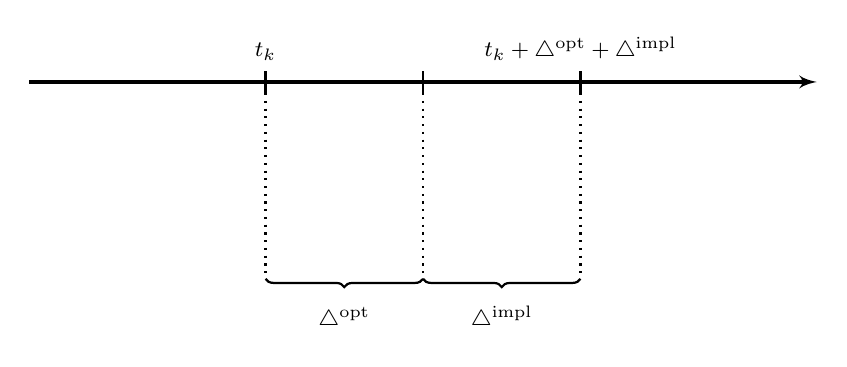
\begin{tikzpicture}[y=1cm, x=1cm, thick, font=\footnotesize]    
    % axis
    \draw[line width=1.2pt, ->, >=latex'](0,0) -- coordinate (x axis) (10,0);       

    % time points
    \draw (3,-4pt) coordinate (t_k)          -- (3,4pt) node[anchor=south] {$t_{k}$};
    \draw (5,-4pt) coordinate (t_k_opt)      -- (5,4pt) node[anchor=south] {};
    \draw (7,-4pt) coordinate (t_k_opt_impl) -- (7,4pt) node[anchor=south]
                                    {$t_{k}+\triangle^{\text{opt}}+\triangle^{\text{impl}}$};

    % curly braces
    \draw[decorate,decoration={brace,amplitude=3pt,mirror}] 
        (3,-2.5) coordinate (t_k_unten) -- (5,-2.5) coordinate (t_k_opt_unten); 
    \node at (4,-3){$\triangle^{\text{opt}}$};
    \draw[decorate,decoration={brace,amplitude=3pt,mirror}] 
        (t_k_opt_unten) -- (7,-2.5) coordinate (t_k_opt_impl_unten); 
    \node at (6,-3){$\triangle^{\text{impl}}$};

    % vertical dotted lines
    \draw[dotted] (t_k)          -- (t_k_unten);
    \draw[dotted] (t_k_opt)      -- (t_k_opt_unten);
    \draw[dotted] (t_k_opt_impl) -- (t_k_opt_impl_unten);
\end{tikzpicture}

\end{document}